\documentclass[tikz,border=8pt]{standalone}
\usepackage{amsmath,amssymb}
\usetikzlibrary{arrows.meta}
\definecolor{latticeblue}{RGB}{28,103,171}
\definecolor{basisred}{RGB}{190,55,55}
\definecolor{diaggreen}{RGB}{36,139,78}
\begin{document}
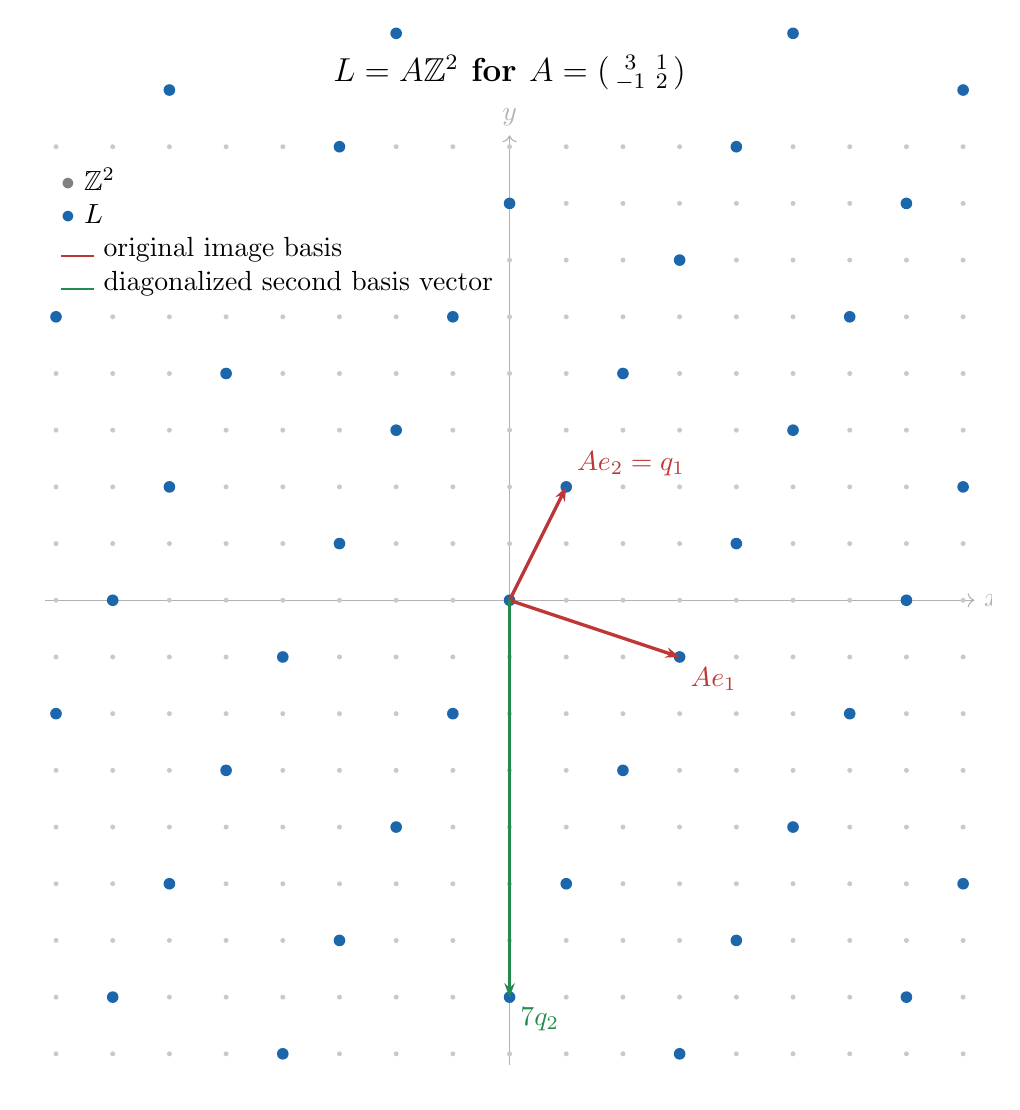
\begin{tikzpicture}[x=0.72cm,y=0.72cm]
  \clip (-8.5,-8.5) rectangle (8.5,10.1);
  \draw[->,gray!60] (-8.2,0)--(8.2,0) node[right] {$x$};
  \draw[->,gray!60] (0,-8.2)--(0,8.2) node[above] {$y$};
  \foreach \x in {-8,...,8}{\foreach \y in {-8,...,8}{\fill[gray!42] (\x,\y) circle (0.9pt);}}
  \foreach \a in {-5,...,5}{
    \foreach \b in {-5,...,5}{
      \fill[latticeblue] ({3*\a+\b},{-\a+2*\b}) circle (2.1pt);
    }
  }
  \draw[-{Stealth[length=5pt]},basisred,very thick] (0,0)--(3,-1) node[below right] {$Ae_1$};
  \draw[-{Stealth[length=5pt]},basisred,very thick] (0,0)--(1,2) node[above right] {$Ae_2=q_1$};
  \draw[-{Stealth[length=5pt]},diaggreen,very thick] (0,0)--(0,-7) node[below right] {$7q_2$};
  \node[fill=white,rounded corners,inner sep=4pt,font=\large\bfseries] at (0,9.3) {$L=A\mathbb Z^2$ for $A=\left(\begin{smallmatrix}3&1\\-1&2\end{smallmatrix}\right)$};
  \node[fill=white,rounded corners,inner sep=3pt,align=left] at (-4.1,6.5) {\textcolor{gray}{\(\bullet\)} $\mathbb Z^2$\\\textcolor{latticeblue}{\(\bullet\)} $L$\\\textcolor{basisred}{\rule{1.2em}{0.7pt}} original image basis\\\textcolor{diaggreen}{\rule{1.2em}{0.7pt}} diagonalized second basis vector};
\end{tikzpicture}
\end{document}
